\documentclass[twocolumn]{article}
%\documentclass[authoryear, 12pt,5p, times]{elsarticle}
%\usepackage[hypcap]{caption}
%\geometry{margin=0.95in,top=1.4in,bottom=1.4in}
%\geometry{margin=1.1in,top=1.5in,bottom=1.5in}
%\textwidth=5cm
\usepackage{appendix}
\usepackage{enumitem}
\usepackage{graphicx}
\usepackage{float}
\usepackage{amsmath}
\usepackage[hidelinks]{hyperref} 
 \usepackage{gensymb}
\usepackage{subcaption}
\usepackage{url}
%\renewcommand\thefootnote{\fnsymbol{\dagger}}
\usepackage[symbol*]{footmisc}
\makeatletter
\newcommand{\rpm}{\raisebox{.3ex}{$\scriptstyle\pm$}}
\begin{document}
%\begin{frontmatter}
%a)              A title page with your name, your partner’s name, the date, and a short abstract (less than 100 words) summarizing your circuit and the results of any measurements.
\title{Final Project: Optical Theremin}\vspace{-20pt}
\author{\today \quad \\Jung Lin (Doris) Lee [Lab Partner: Leah Tom]\\Prof. William Holzapfel, GSI Thomas Darlington, Thomas Mittiga, John Groh,  \\Victoria Xu, Jonathan Ma, Francisco Monsalve, Xiaofei Zhou\vspace{-20pt}}	 
\date{}
\twocolumn[
  \begin{@twocolumnfalse}
    \maketitle
\begin{abstract}
Applying our knowledge from the previous labs about op-amps, transistors, and  diodes, we designed and built an optical theremin that changes the frequency and amplitude of the sound output based on the amount of light incident on the device. The main circuit consists of bandpass filters, inverting amplifiers, and full wave rectifiers to perform the frequency and amplitude modulation, with a JFET modulator is used to combine output result. Various circuit modifications described in this report improved the performance of our modulation control, which enabled us to attain a distinctly audible dynamic range of 2V and frequency range of 1 octave. %ahat we implemented and demonstrate how they improved the performance of the modulation control and the audio quality of the theremin.  % In this report, we describe the reasoning behind the 
 \end{abstract}
  \end{@twocolumnfalse}
]\maketitle
\section{Introduction}
%b)              A one-page introduction.
% gained popularity in media ,
Theremin is a type of electronic musical instrument that can be played without the performer touching the instrument. Their eerily-sounding tunes gained media popularity in 1940s movie soundtracks and pop and rock music, after Leon Theremin first invented the device in 1920. Most existing implementations of theremins consist of two metal antennas operating at radio frequencies. The performer's hand acts as a variable capacitor between the antennas and the grounded plate, determining the frequency of the oscillator circuit and thereby, controlling the volume and pitch of the output audio signal.
%changes the distance .
\par Our project was initially inspired by  Bonnie Eisenman's \textit{Illumaphone} project {\footnotesize[7]}, an optical theremin with 6 light cups as ``piano" keys tuned to 6 different octaves.  A brief literature search showed that most DIY optical theremin projects contains relatively simply circuitry of only a single photoresistor whose output is fed to a microcontroller. These approaches avoids the hassle of doing signal processing and filtering on the hardware level and leaving most of the work to the music processing software. We distinguish our project from these prior works by designing a optical theremin that takes an entirely hardware-based approach to encompasses all the signal acquisition, filtering, processing, and audio output steps. 
\par Our design concept motivated us to include noise-reducing modules such as the bandpass filters, in sync with the relaxation oscillator's output frequency for the LED. The challenging task of achieving audible sounds was attained by carefully designing appropriate inverting amplifiers and push-pull output stage. %series of ---- voltage controlled oscillator and ----- inverting amplifiers
Although we are unable to achieve as much as the dynamic range and smooth sound quality as the \textit{Illumaphone} with this entirely hardware-based approach, we have  sufficiently achieved our design objectives for this project by achieving a distinguishable dynamic range for frequency and amplitude modulation.
\section{Circuit Description}
\subsection{Functional Description}
%i)                Start with a functional description: a block diagram listing all the major operations in your circuit.
\begin{figure*}
 \centering
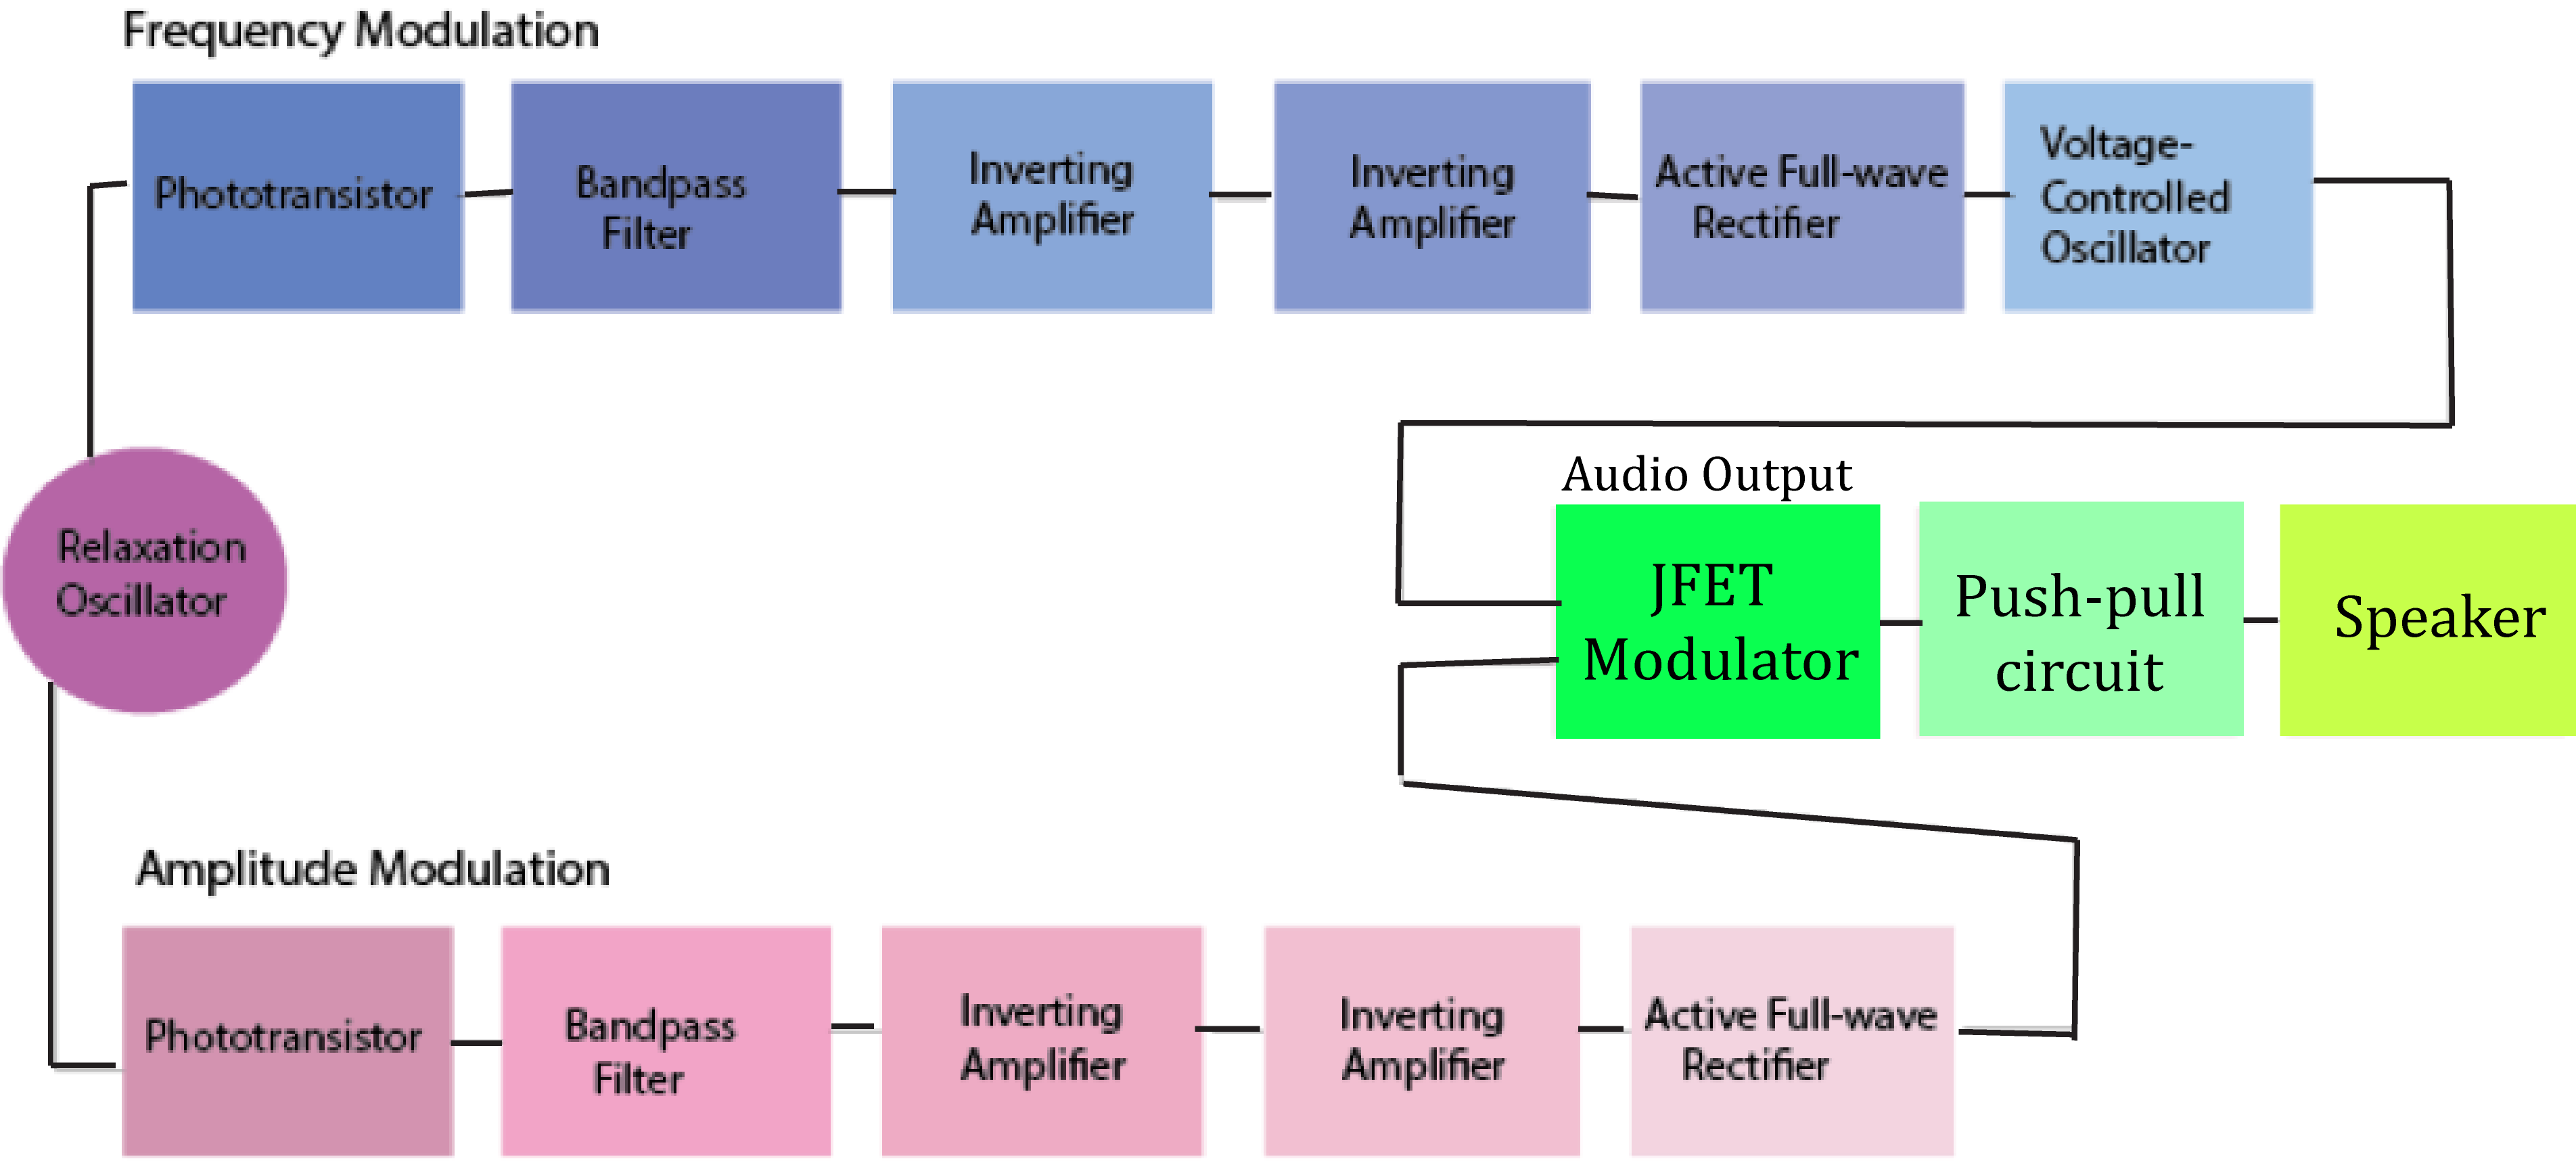
\includegraphics[width=450pt]{figure/block}
\caption{Block diagram of circuit modules. }
\label{block}
\end{figure*}
\par At a high level, the device can be broken down into three subcircuit: one responsible for amplitude modulation (denoted in red in Fig.\ref{block}), one for frequency modulation (blue) and one for audio output(green). 
\par We first computed a rough estimate for the resistance and capacitance for each module based on the calculations and simulations detailed in the next section. Then, we built the circuit using these values and test for their performance, in some cases, we had to change the computed values by testing different values that yields better results. Our final, working circuit design is shown in Appendix A.
\subsection{Component Description}
%iii) A description of the purpose and operation of all the major components in the circuit (most likely all the active components and some of the passive components.)  Relate each major component to the appropriate function block.
\subsubsection{Phototransistor}
\par We used an OP802SL NPN phototransistor connected to an op amp to detect the vertical position of the performer's hand, based on the amount of red LED light incident on the phototransistor. Initially, we used a photoresistor to detect our optical signal. Even though the photoresistor gave a sufficiently large range (267$\Omega$ to 4.353k$\Omega$) of continuous signal change, there was significant lag between the circuit signal response shown on the oscilloscope relative to when we actuated the change. 
\par The phototransister improves the performance of this detection module by resolving the lagging issue seen with the photoresistors. We had a lot of difficulty in testing whether the phototransistor gave a response, so we began by first building a test circuit where we attached a 12V power supply to the collector and the measuring the output on a oscilloscope to detect a response. As detailed in section \ref{photo}, we determined that the phototransistor had an approximately linear response to its separation distance from the red LED. We chose to use a red LED because its wavelength is closer to the peak on the spectral response graph than the other color LEDs, as detailed in the OP802SL spec sheet {\footnotesize[8]}. Since changing the light incident on the detector is what varies the base-emitter voltage, the base should be connected to nothing, as denoted in most schematics on phototransistor spec sheets. \footnote{In fact most manufacturer sells two-pronged, phototransistors without the base.}  
\subsubsection{Bandpass filters}
The bandpass filters in our circuit is designed to eliminate interference from ambient light sources. To enforce this stringent conditions, we initially designed the filters to pass through signals of frequencies between 900 and 1100 Hz. Using a 1$\mu$F capacitor, we computed the resistance values as: 
\begin{align*}
f = \frac{1}{2\pi RC}
\\ R = \frac{1}{2\pi (1.0\times10^{-6} F)f}
\end{align*}
However, we found that the signal that passes through was too low. Careful consideration of the main noise sources such as the fluorescent lighting (60Hz) shows that enforcing narrow 200Hz window is not necessary. Therefore, we relaxed the range of the filters to 500$\sim$2000 Hz. (R = 82$\pm 4.1\Omega$ and 300$\pm15\Omega$)
\subsubsection{Inverting Amplifer}
\par Since the phototransistor was connected in series with an op amp, the signal output from the detection module is very small (100mV$\sim$1V range). So, we built two inverting amplifiers to step up the signal  before it is fed into the rectifier. First, we used the unmodified design from Lab 6 with  R1= 47k$\Omega$ resistor , but we found that the $V_{out}$ only rails as we cover up the phototransistor. In order to map out a more detectable change, we increase the gain by decreasing the value of R1 to 1k$\Omega$, since
\begin{equation}
V_{out} = -R_2I = \frac{-R_2V_{in}}{R_1}
\end{equation}
where the gain is -R2/R1. Testing these modules, we use two 1$\mu$F capacitor to decouple the power supply and minimize the parasitic oscillation. 
\par As shown in our final circuits in Fig.\ref{freq_circuit} and \ref{amp_circuit}, the \texttt{Inverting Amplifier I}  has a gain of $R_2/R_1 =  100k\Omega/1k\Omega=100$. \texttt{Inverting Amplifier II} has a gain of $R_2/R_1 =  330\Omega/100\Omega=3.3$. Multiplying the effect of these two amplifier when connected in series gives us an overall signal amplification of 330. 
\subsubsection{Full Wave Rectifier}
\begin{figure}[h!]
 \centering
 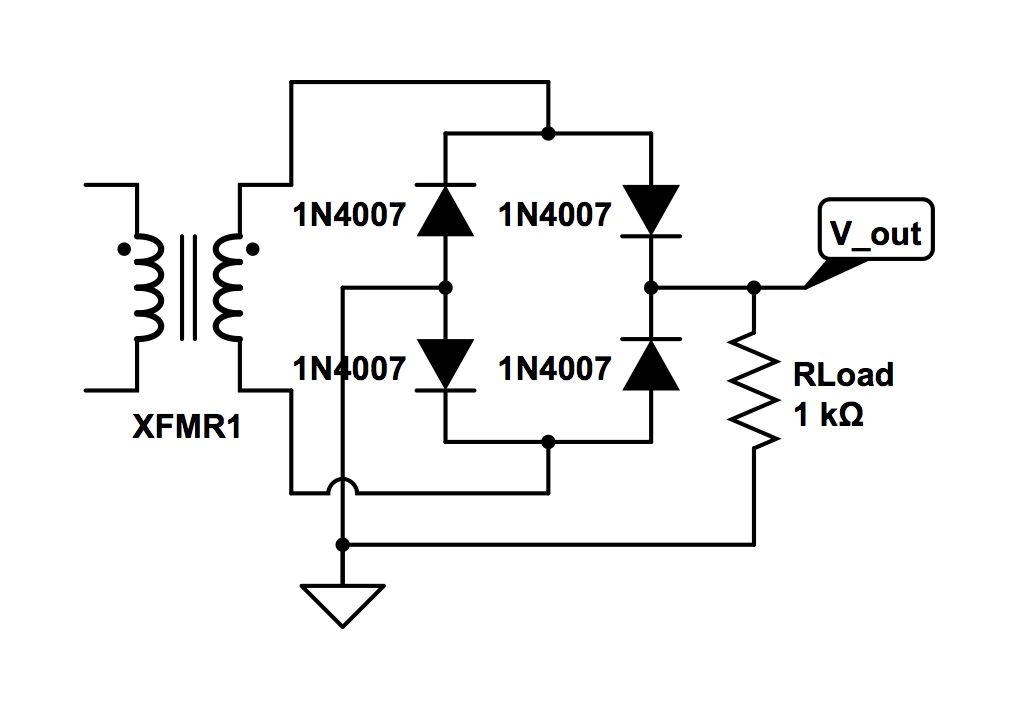
\includegraphics[width=220pt]{figure/full_wave_rectifier.jpg}
\caption{Common implementation of full-wave rectifier. {\footnotesize[3]}}
\label{rectifier}
\end{figure}
The full wave rectifier that we built is a modified implementation of a Graetz bridge with four 1N4007 diodes. As shown in Fig.\ref{rectifier}, these devices are commonly hooked up to the output of a transformer. But for our purpose we simply hooked up a waveform generator signal to test how the rectified signal looks like, as shown in \ref{full_wave_scope}. Since the diode only passes through current in one direction, the arrangements of diodes, passes through the positive current and flips the negative signal up. In addition, we inserted a smoothing capacitor to give an output of DC. The smoothing capacitor takes the ripple voltage of the rectified waveform in order to flatten the oscillating output of the full-wave rectifying circuit  to give a DC voltage. This DC voltage is what is fed into the JFET modulator. We also removed the load resistor to minimize dissipation.  
\begin{figure}[h!]
 \centering
 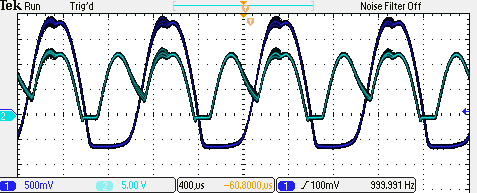
\includegraphics[width=220pt]{figure/full_wave_scope.PNG}
\caption{Channel 1 shows the original sinusoidal signal being fed into the scope, Channel 2 shows the signal rectified by the full-wave rectifier circuit. }
\label{full_wave_scope}
\end{figure}
\par As seen in Fig.\ref{full_wave_scope}, even though the rectifier effectively flips the negative signal up, there is still a gap between the subsequent signals. The gap is about a sixth of the wavelength of the signal, so this is still better than what a half-wave rectifier would output. After testing with the audio output, we found that even though the frequency change is distinguishable, the output response sounded discretized. We suspect that this effect of crossover distortion may be one of the contributing factor that degrades the audio quality of the output signal.
\par Therefore, we decide to switch to an active rectifier composed of two op amps to perform the full wave rectification on our frequency modulation circuit.  Unlike in the frequency modulating circuit, amplitude variation responds and outputs a continuous change and is unaffected by the passive rectifier. Therefore, we kept with the four-diode, passive full-wave rectifying circuit in our amplitude modulating circuit. 
\subsubsection{Voltage Controlled Oscillator}
\begin{figure}[h!]
 \centering
 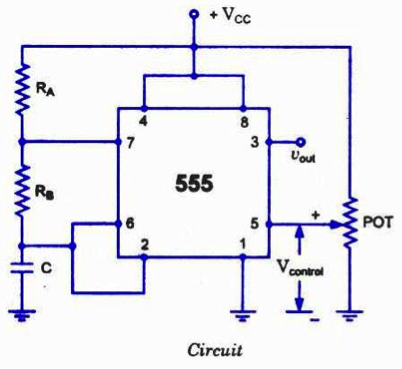
\includegraphics[width=220pt]{figure/vco.png}
\caption{Voltage Controlled Oscillator}
\label{vco}
\end{figure}
The voltage-controlled oscillator plays a central role in the frequency modulation circuit in converting the input DC voltage to a signal waveform. The frequency of the output audio wave is described by Eq.\ref{vco_eq}:
\begin{equation}
f = \frac{1}{(R_1+R_2) C ln \frac{V_{cc}-V_{con}}{V_{cc}-0.5V_{con}}}
\label{vco_eq}
\end{equation}
where $V_{cc}$ is the +12V used to power the 555 Timer. Initially, we used a 1$\mu$F capacitor and set $R_1=20k\Omega$ and $R_2=2k\Omega$ to get a control voltage of 2V and 8V, corresponding to a frequency of 1000Hz and 6000Hz. However, we wanted a VCO that would give us the frequency response for a control voltage between 0 to 10V. So as shown in the Fig.\ref{freq_circuit} circuit, we included additional amplifiers that feeds into the control pin of the 555 Timer in order to get to that range.
\subsubsection{JFET Modulator}
In order to effectively combine the DC output from the amplitude modulation circuit with the VCO-generated waveform from the frequency modulation circuit, we built a JFET modulator as shown in Fig.\ref{audio_circuit}. At first, we tested the modulator independent of the rest of our circuit by simply feeding in a input carrier wave of 1MHz  from the waveform generator. Using another function generator to drive the a 1kHz, 1V$_{pp}$ sine wave on the potentiometer gate signal, we find that the input carrier wave  is modulated by the 1kHz wave as shown in Fig.\ref{q9trace}.
 \begin{figure}[h!]
 \centering
 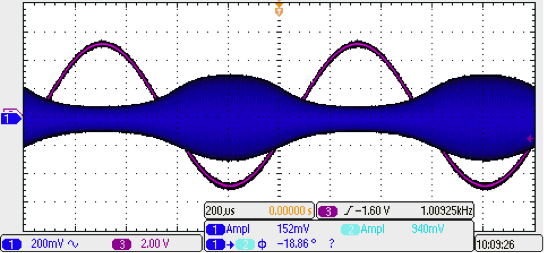
\includegraphics[width=0.5\textwidth]{figure/q9trace}
\caption{Scope traces for the AM signal. Channel 1 shows the modulated $V_{out}$, whose amplitude has a lower resulting amplitude than the 1kHz signal in Channel 3.}
\label{q9trace}
 \end{figure}
\par  After adjusting the potentiometer values, the circuit successfully modulates the DC output amplitude by the frequency waveform on our theremin circuit. However, we increased the value of $R_{drain}$ from 1k to 10k$\Omega$ to boost up the signal output. Despite this, external amplification of this output was still necessary to create an audible signal. 
\subsubsection{Push-pull Output Stage}
Since the audio signal that we ended up getting from the multiplier is in the millivolts range, it can not be mapped onto an audible signal on the speaker. We tried to boost up this signal by building a high gain inverting amplifier. However, since the output voltage of the op amp is current-limiting, we can not simply use an inverting amplifying to perform this task. Instead, we use a push-pull stage from Lab 8 to increase the current gain of the input signal by making use of BJT as current amplifiers. As seen in Fig.\ref{audio_circuit}, the 51k$\Omega$ resistor acts as feedback to minimize the crossover distortion when the signal is passes from the upper BJT to lower BJT, leading to better audio quality.
\subsubsection{Relaxation Oscillator}
We use a relaxation oscillator to generate the ``On-Off signal" for the LED flashing at 1kHz.The output frequency of the circuit is described by :
\begin{equation}
f=\frac{1}{2 R_f C ln\frac{1+\beta}{1-\beta}}
\end{equation}
where $\beta$ is the ratio of the resistances $\frac{R_3}{R_3+R_2}$.
\begin{figure}[h!]
 \centering
 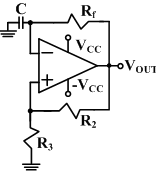
\includegraphics[width=120pt]{figure/relax_osc.png}
\caption{Relaxation Oscillator Schematic.}
\label{relax_osc}
\end{figure}
\par Initially, we built the circuit using the combination of $R_f$ = 100$\Omega$ and $R_3 = 100\Omega$, C=1000$\mu$F and $R_2 = 3 M\Omega$. However, we found that the output frequency deviate largely from our computed frequency of 10Hz (initially designed for the photoresistor circuit). We suspect that this is due to our use of a the large 1000$\mu$F electrolytic capacitor. After trying different combinations of resistances and capacitance, we found that the circuit yields optimal performance when $R_2$ and $R_3$ are approximately equal. %and using a 1$\mu$F non-electrolytic capacitor. 
\par This new approach simplifies the calculation so that no matter what $R_2$ and $R_3$ is chosen to be the $\beta$ is still 0.5. In our final design, we chose $R_2$ and $R_3$ to be 1k$\Omega$, with C=10$\mu$F. The computed $R_f$ served as a convenient baseline for us to then fine-tuned the resistance so that we achieve the 1kHz signal as measured by the oscilloscope shown in \ref{relax_osc_b4boost}.
\begin{figure}[h!]
 \centering
 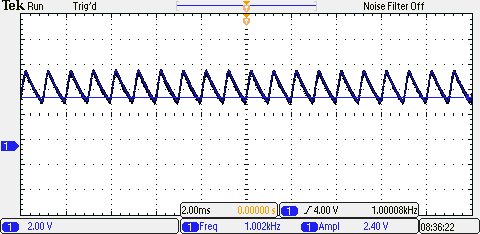
\includegraphics[width=220pt]{figure/relax_osc_beforeboost.png}
\caption{1kHz signal generated by the relaxation oscillator.}
\label{relax_osc_b4boost}
\end{figure}
\par Although the output voltage is suppose to switch from positive to negative $V_{cc}$, we found that the output voltage was only around 1.6V, which was below the turn on voltage of the LED. We tried using the signal as a switch with an additional 5V with a resistor to ``boost up" the signal to the LED, but had trouble figuring out how to arrange the activation signal with respect to the output LED and the rest of the circuit the for this purpose. By building an amplifier connecting to the output of the relaxation oscillator, we were able to attain a output voltage of around 3V while retaining the 1kHz signal.
\par When soldered together, this circuit served as a convenient module that can be easily moved to change the light incident on the detector, without the bulkiness of the waveform generator.


\section{Experiment and Results}
%f)                A description of the experiments you performed with your circuit and the measurements you made, including your experimental methods, your raw data (in tabular or graphical form), and data and error analysis.
\subsection{VCO Simulation}
Prior to building the VCO and testing with values in Eq.\ref{vco_eq}, we simulated the response of the VCO on CircuitLab to get an order-of-magnitude estimate for the voltage input range that was required to get the desirable output frequency.
\begin{figure}[h!]
 \centering
 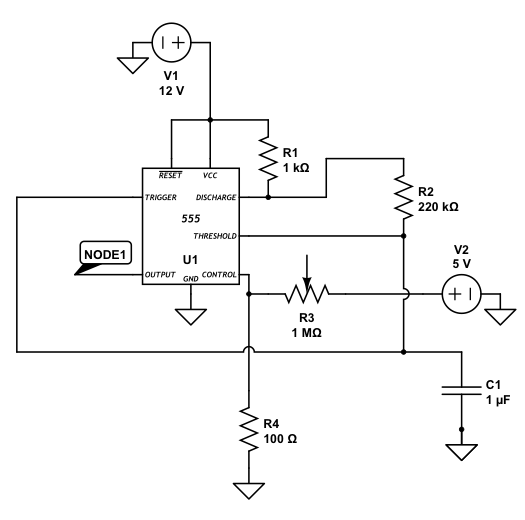
\includegraphics[width=230pt]{figure/vco_sim.png}
\caption{VCO circuit simulation setup.}
\label{vco_sim}
\end{figure}
\par We connected the control voltage to the $R_3$ and $R_4$ voltage divider  and a 5V power supply. As we vary the resistance value for $R_3$, transient analysis was conducted on the output (\texttt{NODE1}) on the 555 Timer. Reading off the time per cycle between pulses in Fig.\ref{sim_vco_r3}, we get a sense of the frequency output of the VCO. 
 \newpage
\begin{figure}[h!]
 \centering
 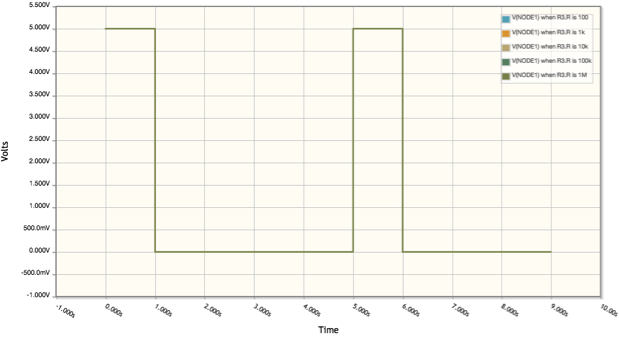
\includegraphics[width=230pt]{figure/sim_1m.png}
\end{figure}
\begin{figure}[h!]
 \centering
  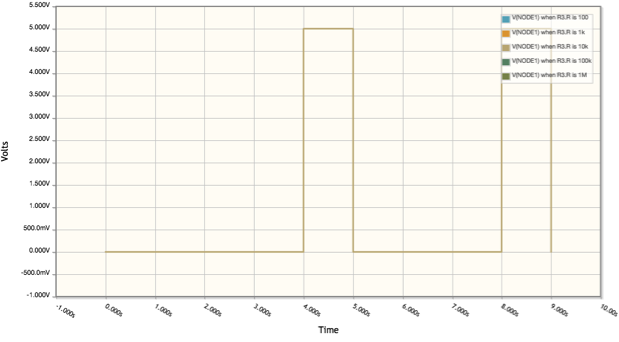
\includegraphics[width=230pt]{figure/sim_10k.png}
\end{figure}
\begin{figure}[h!]
 \centering
   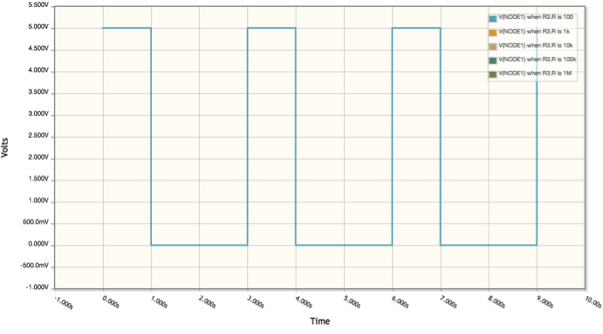
\includegraphics[width=230pt]{figure/sim_100.png}
\caption{Transient analysis for $R_3$ = 1M$\Omega$(Top), 10k$\Omega$ (Middle), 100$\Omega$ (Bottom).}
\label{sim_vco_r3}
\end{figure}
\newpage
\subsection{Calibrating Phototransistors\label{photo}} 
\par The current varies with varying light intensity and this translates to a proportional voltage at the output of the op-amp due to the resistor across the op-amp.   continuous instantaneous circuit response,
Approx linear response as expected since inside operating region, use for calibrating theremin. 
\begin{figure}[h!]
 \centering
 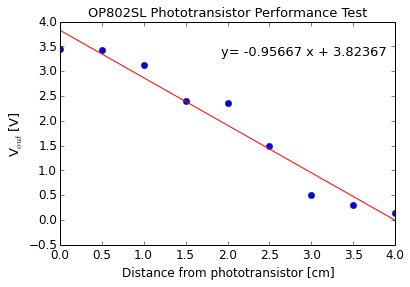
\includegraphics[width=220pt]{figure/phototransistor_performance}
\caption{Quantify the performance of the phototransistor by varying its separation distance from a red (660nm), 1kHz, 4V$_{Vpp}$ LED source.}
\label{phototransistor_performance}
\end{figure}
\subsection{Measurements and Results}
\begin{figure*}
 \centering
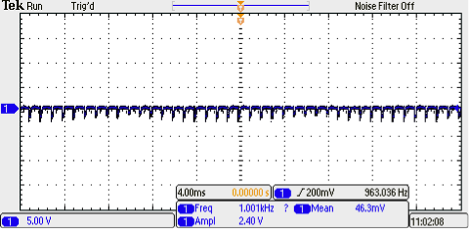
\includegraphics[width=220pt]{figure/a1}
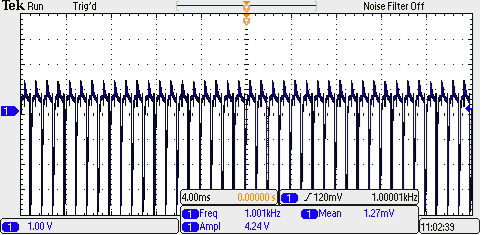
\includegraphics[width=220pt]{figure/a2}
\caption{Performance of the amplitude modulation circuit. Left: Separation distance of 4 cm. Right: Separation distance of 0 cm.}
\label{a}
\end{figure*}
Our final circuit yields a modulated audio signal at normal hearing level.  As we varied light incident on the frequency modulation circuit and fixed the amplitude, we achieved a frequency range of about one to two octaves. When the LED was furthest from the phototransistor, the frequency was 500Hz. As it was brought as close as possible, the frequency then became 2.6kHz as shown in graphs below. The signals look different for when the frequency was modulated and the amplitude was modulated because the amplitude modulation LED was held some distance away as the frequency LED was varied and the noise inherent in the circuit makes the signal look different.
\begin{figure}[h!]
 \centering
 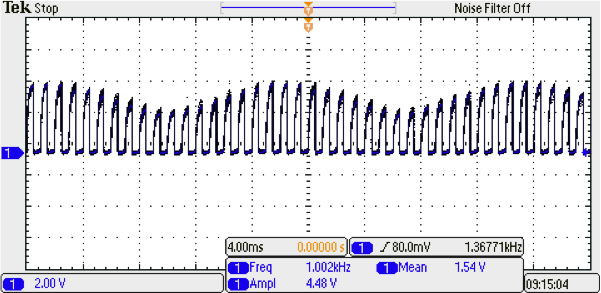
\includegraphics[width=220pt]{figure/octave}
\caption{Scope traces of the modulated waveform output.}
\label{octave}
\end{figure}
\par  When the frequency is kept fixed and the light incident on the amplitude modulation circuit is changed, we were able to get a the sound from vary from sounding very loud to very quiet on human hearing level. The corresponding dynamic range in voltage is about 2V as shown in the Fig.\ref. The amplitude of the output wave when the LED is at its maximal separation distance is 2.40V. The amplitude increases to 4.24 V when the phototransistor is set to its minimal separation distance (i.e. touching the surface of the phototransistor). 
\begin{figure*}
 \centering
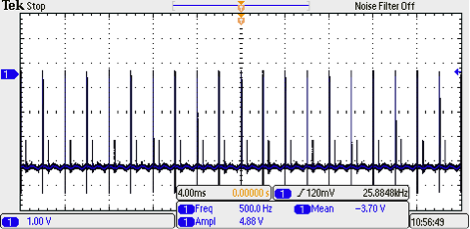
\includegraphics[width=220pt]{figure/f1}
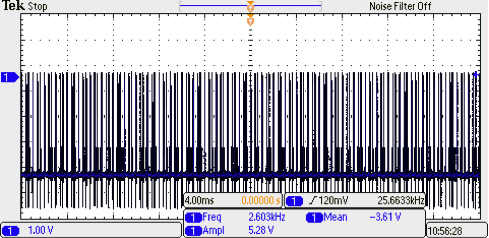
\includegraphics[width=220pt]{figure/f2}
\caption{Performance of the frequency modulation circuit. Left: Separation distance of 4 cm. Right: Separation distance of 0 cm.}
\label{f}
\end{figure*}
\par The limiting factor in the detection module is that even at maxiumum operating level the LED brightness is simply too low for the phototransistor to detect beyond a separation distance of 4cm. This could be improved by building a light funnel around the phototransistor or replacing the LED with a larger bulb flashing at 1kHz. \footnote{We attempted to do this with aluminum foil,  since we thought that the reflective surface would act as a wave guide for the LED's light to travel. However, we ended up shorting our LED multiple times since the foil is conductive.}  When varied together, interesting combinations of sound can be made and ,in theory, we can probably play a simple musical tune with this device.
%attain a distinctively audible dynamic range of 5V and frequency range of 1 octave.
\newpage
\section{Conclusion}
%g)              Conclusions.
\par In this report, we describe an entirely hardware-based optical theremin capable of achieving an audible dynamic range of 2V and frequency range of one to two octaves. The optical theremin works by detecting the light intensity change actuated by the performer's hand motion. Using a relaxation oscillator to pulse the LED at 1kHz, a set of bandpass filters windowed at that frequency picks up this signal and feeds it into a full wave rectifier to make the signal positive. In the freqeuncy modulation circuit this DC voltage is fed into a voltage controlled oscillator, yielding a frequency modulation waveform. Finally, a JFET modulator is used to combine output result and feed the audio signal to a speaker.
\par  Contrary to our simplistic initial design, many new functional modules were added to optimize the performance of our modulation control. We learned about the disadvantages of using a diode-bridge, passive full wave rectifier and addressed the need for inverting amplifiers to generate a detectable signal.  In addition, we found that a push pull output stage is necessary for stepping up our output signal to the audible range.  Possible future improvements on this circuit includes modifying the op-amp circuit setup connected to the phototransistor, increasing the sensitivity of the theremin at larger separation distance, and mapping the input signal onto a greater range of frequency outputs.
\newpage
\section*{Acknowledgments}
\begin{footnotesize}
The author would like to acknowledge support from the GSI and Professor Holzapfel in this lab in addressing our questions about how the circuits work, assisting us with the initial circuit design, and suggesting ways to improve its performance.  We also appreciate helpful discussion and debugging assistance from Elijah Campbell's group that helped this work.
\end{footnotesize}
  \section*{References}
 \begin{footnotesize}
\begin{enumerate}[label={[\arabic*]}]
\setlength\itemsep{0.001em}
 \item Horowitz, Paul, and Winfield Hill. \textit{The Art of Electronics}. Cambridge: Cambridge UP, 1989. Print.
 \item ``Lab 5 - JFET Circuits II. " \textit{Donald A. Glaser Advanced Lab.} Regents of the University of California, n.d. Web. 01 May. 2015.
 \item Nichole. "Create a DC Power Supply." \textit{Instructable}. N.p., n.d. Web. 1 May 2015.
  \item `` Lab 8 - Op Amps III " \textit{Donald A. Glaser Advanced Lab.} Regents of the University of California, n.d. Web. 07 May. 2015.
  \item ``Lab 12 - Final Project " \textit{Donald A. Glaser Advanced Lab.} Regents of the University of California, n.d. Web. 07 May. 2015.
 \item ``Op-amp Relaxation Oscillator." \textit{Electronic and Electric Circuit Simulation.} N.p., n.d. Web. 9 May 2015.
 \item Eisenman, Bonnie. "Illumaphone: Light-based Musical Instrument with Arduino." \textit{Instructables}. N.p., n.d. Web. 10 May 2015.
 \item ``NPN Silicon Phototransistor." \textit{OPTEK} (1996): n. pag. Web. 12 May 2015.
\item  ``Optical Sensors - Photo Detectors - CdS Cells." \textit{DigiKey}, n.d. Web. 12 May 2015.
 \item ``Theremin." \textit{Wikipedia}. Wikimedia Foundation, n.d. Web. 12 May 2015.
\end{enumerate}
  \end{footnotesize}
%\subsubsection{Photoresistor Calibration}
%\begin{table}
%    \begin{tabular}{l|l}
%                                 & Resistance [$\Omega$] \\ \hline
%	Dark                          & 4.353k     \\ \hline
%    Ambient Light                 & 1.205k     \\ \hline
%    RED LED (3V)  & 267.3      \\ 
%    \end{tabular}
%    \label{photor}
%    \caption{Photoresistor resistance range for different light setting.}
%\end{table}
\onecolumn
\section*{APPENDIX A : Circuit Diagrams for Major Modules}  
%\twocolumn[\@twocolumnfalse
%\section*{APPENDIX A : Circuit Diagrams for Major Modules}  
%  \centerline{\Large\bfseries This is my manually set ``wide'' title}
%  \vspace{3ex}
  % ]\maketitle
\begin{figure*}[h!]
 \centering
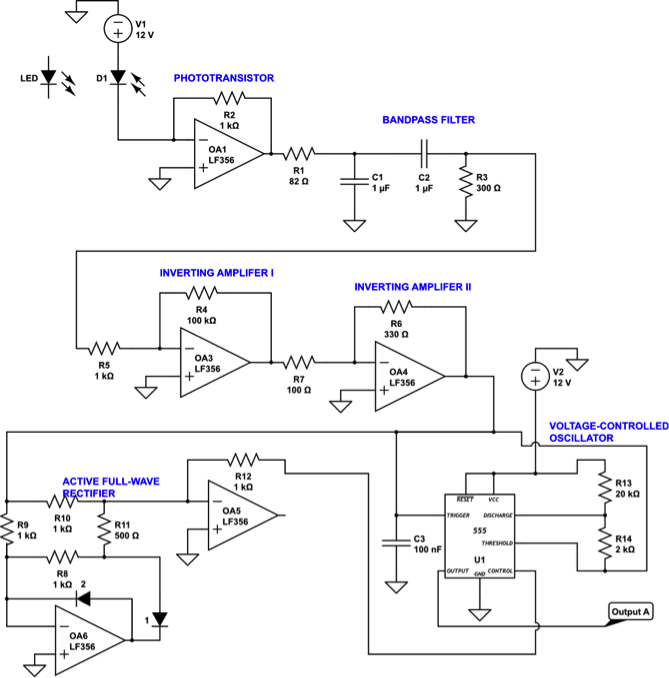
\includegraphics[width=440pt]{figure/freq_circuit}
\caption{Frequency-Modulating circuit.}
\label{freq_circuit}
\end{figure*}
\begin{figure*}[h!]
 \centering
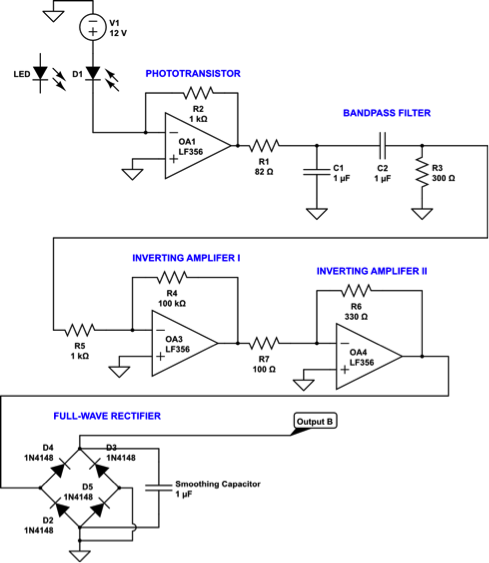
\includegraphics[width=280pt]{figure/amp_circuit}
\caption{Amplitude-Modulating circuit. Note its similarity to the frequency modulation circuit, with the addition of the VCO module. }
\label{amp_circuit}
\end{figure*}
\begin{figure*}
 \centering
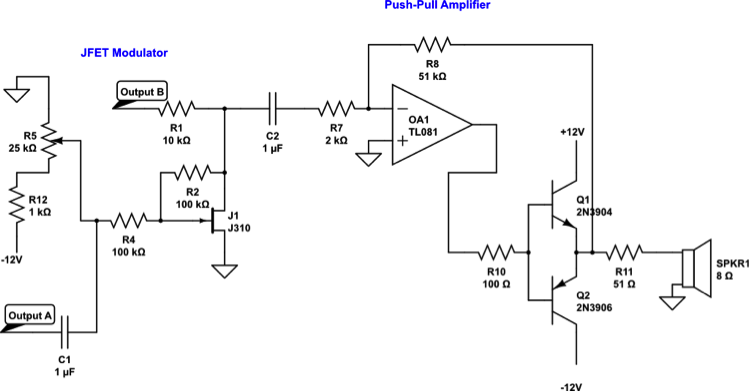
\includegraphics[width=280pt]{figure/audio_circuit}
\caption{Audio output circuit.}
\label{audio_circuit}
\end{figure*}
\end{document}